\chapter{3D Model Building}
This chapter describes how to build a generative textured 3D face model from an example set of 3D face scans. A morphable model is derived from the set of scans by transforming their shape and texture into a vector space representation. The term generative implies that new faces can be generated by calculating linear combinations of the set of examples. 

\section{3D Morphable Model}
The 3D Morphable Model (3DMM) published by Blanz and Vetter in 1999 (bib) is a multidimensional function for modelling textured faces derived from a a large set of $m$ 3D face scans. A vector space can be constructed from the available data set where each face is represented by a shape-vector $S \in \mathbb{R}^{3n}$ that contains a stack representation of its $n$ vertices. The texture-vector $T \in \mathbb{T}^{3n}$ contains the corresponding RGB values. New shapes and textures can now be computed
with a linear model parametrized by barycentric shape $\vec\alpha \in \mathbb{R}^{m}$ and texture coefficients $\vec\beta \in \mathbb{R}^{m}$.\\
However, the goal of such a 3D face model is not just to construct arbitrary faces, but plausible faces. This is achieved by estimating two multivariate normal distributions for the coefficients in $\vec\alpha$ and $\vec\beta$.
By observing the likelihood of the coefficients it is now possible to find out how likely the appearance of a corresponding face is.
The multivariate normal distributions are constructed from the average shapes $\overline{S} \in \mathbb{R}^{3N}$ and textures $\overline{T} \in \mathbb{R}^{3N}$ of the datasets and the covariance matrices $K_{S}$ and $K_{T}$, which are defined over the differences between each example and the average in both shape and texture.
The covariance matrices are then used to perform a Principal Component Analysis which defines a basis transformation to an orthogonal coordinate system the axis of which are the eigenvectors of the respective covariance matrices.

\begin{equation}
\label{eq:MM}
\mathcal{S}(\vec\alpha)=\overline{S}+S\vec\alpha, \quad \mathcal{T}(\vec\beta)=\overline{T}+T\vec\beta
\end{equation}

In \eqref{eq:MM} the $N=m$ principal eigenvectors of $K_{S}$ and $K_{T}$ respectively are assembled column-wise in S and T and scaled in a way such that the prior distribution over the shape and texture parameters is given by a multivariate normal distribution with unit covariance (Amberg).

\begin{equation}
    p(\vec\alpha, \vec\beta) = \mathcal{N}(\vec\alpha\vert|\vect{0}, \mathbb{I})\mathcal{N}(\vec\beta\vert|\vect{0}, \mathbb{I})
\end{equation}

\section{Achieving Correspondence through Registration}
\viscomment{be as specific to say there are triangulated meshs?}
In order for a 3D Morphable Model to generate plausible faces we have to make sure that all faces in the example set are parametrized equally. For this reason the meshs first have to be brought into correspondence, which is the case when the vertices of different meshs which are at the same semantical position, i.e the left corner of the left eye, have a similar vertex number. A dense point-to-point correspondence between two meshs is accomplished through the process of registration.  
\begin{comment}
meaning that all faces share the same mesh triangulation, respectively the vertices at the same semantical position, i.e. the corner of the eye, have a similar vertex number. Correspondence is achieved/accomplished through the process of registration.
\end{comment} 
The training data used for learning a 3D Morphable Models consists solely of registered examples of the 3D shape and texture of faces.

incorporate
\textit{WE WANT POINT TO POINT CORRESPONDENCE BETWEEN THE TWO FACES
in general: point to point correspondence between to images
Are scans already in semantical correspondence? No semantical correspondence
FINDING CORRESPONDENCE IS EXACTLY THE AIM OF REGISTRATION => HAVING SAME POINTS AS CLOSE TO ONE ANOTHER AS POSSIBLE
Now in order to obtain a 3D representations of the face we need to transform the mean face so that it fits a particular 3D face scan. To find the transformation, however, we first have to find feature points in both 3D representations which correspond to the same semantical structure. Previous work has shown that point landmarks are not sufficient to preserve the level of detail which is imminent in the regions of the eyes, ears and lips and that the computed transformations are not able to preserve these regions. For this reason, additional line features have been introduced. In order to relate these 
How registration works so far
What we want to change}
\paragraph{Registration Algorithm}
Registration is the task of parametrizing one shape in terms of another shape so that the points which are semantically correspondent are mapped onto each other. From a different viewpoint the parametrization can be viewed as a deformation. The shape which is deformed is called the template or reference shape, while the goal shape of the mapping is called the target shape. 
Registration achieved using a Registration algorithm.
Such an algorithm uses prior information in the form of manually clicked feature points, so called landmarks, on all of the face meshs. Correspondence in-between these points is defined through smooth deformations of the template mesh which match the surface and feature points of the target. 
In this thesis we introduce \viscomment{``use'' better? It is already academically introduced, just not in this context} a registration algorithm which is novel to the problem of 3D face registration in two ways: the use of prior information is extended to whole contours of complex regions of the face, refered to as line features and the deformation is modeled using Gaussian Process Regression, a
method from the field of Machine Learning.

\section{Prerequisite Data}
image with landmarks and line features
a short overview what data we have given

Facial Scans:
face scans given as point clouds
The data we have given is a set of about 300 face scans that have had a set of key points marked. Furthermore important and detailed regions like the eyes, ears and lips have been marked by contour lines known as line features. The scans have been obtained with a … scanner. The surface is very detailed, however the eyes and the nostrils are not recorded. From these scans we want to create fully textured 3D faces, which can be used to build a new face model.

Mean Face:
The mean face has been derived from a collection of 100 male and 100 female 3D face models.
\begin{figure}
\centering
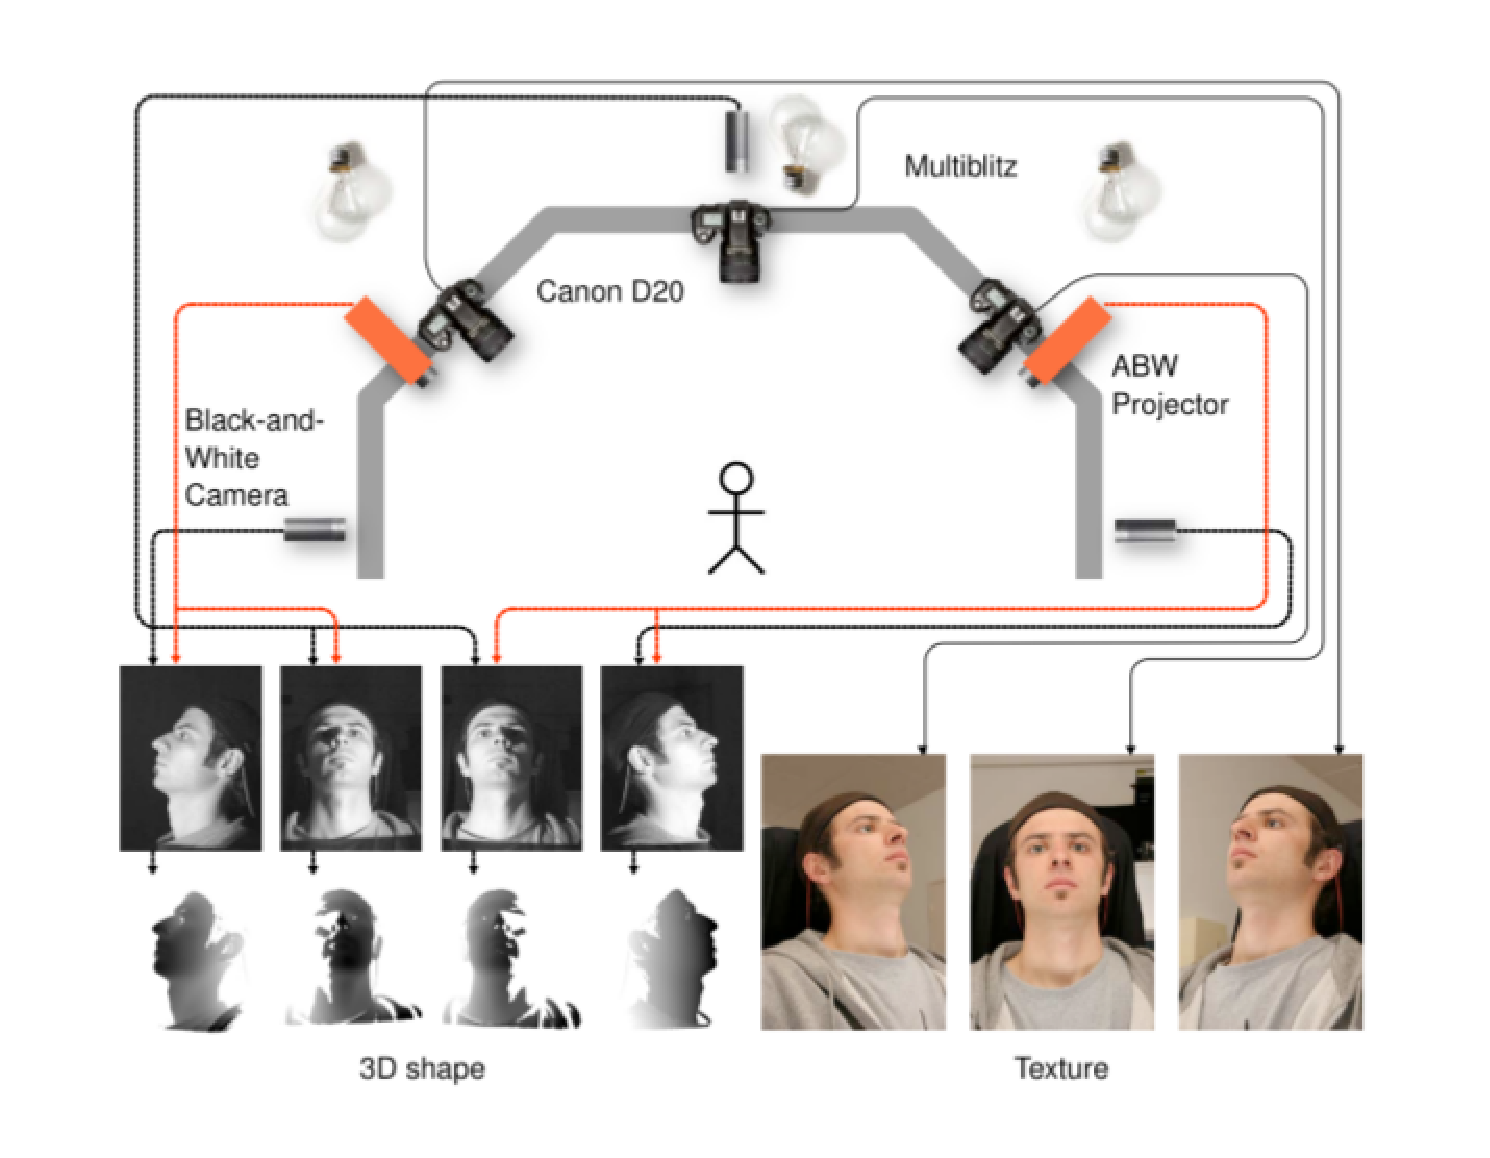
\includegraphics[width=\textwidth]{./resources/figures/scanner.eps}
\caption{3D scanner}
\label{fig:scanner}
\end{figure}
Describe data and scanner given + Camera model?
In the next chapter we will elaborate on the approach of using Gaussian Processes to solving the problem 3D face registration.

\nopagebreak



